\chapter{The \texttt{X10ABOT} Architecture, Design and Implementation}% (fold)
\label{cha:the_x10abot_architecture_design_and_implementation}


In this chapter we describe how we used the design strategies which were introduced in the background chapter. We extracted the most compelling features and combined them to crate a modular system with the following components which comprise the \xten architecture:
\begin{enumerate}
\item The Motherboard
\item The Daughterboard
\item The Peripheral Bus
\item Input and Output Ports
\item The Motherboard Library
\item Daughterboard Firmware
\item The Middleware
\end{enumerate}

%\section{Physical Setup} chapters should represent compoents of the system

% Chapter 3

%%Impact or influence of the design decisions and how they were implemented
The \xten 's main architectural features that were decided on were modularity, scalability and extensibility. It was also important that we kept the cost of implementation relatively inexpensive. These attributes represented common design patterns observed over a number of robotics projects, either for custom robots or as a part of the architecture for general purpose robotics kits. We designed a system which comprises of components which realize one or more of the design requirements.

%User friendly:  Usable primary school to  graduate level roboticists
\newpage
\section{The Architecture} % (fold)
\label{sec:the_architecture}
Based on the design requirements listed in the previous chapter, we created an architecture that captures all the previously listed features without making any significant compromise on any of those aspects. The \xten architecture meets all the previously outlined requirements at both the hardware and software level. It is comprised of a motherboard, the main central controller and the head of a distributed system of peripheral sensor and actuator boards called daughterboards that carry out a standard set of computations synonymous to a thin client, all connected across the central peripheral bus. The motherboard coordinates and controls all operations on the entire system and all operations are either initiated or terminated at the motherboard. The motherboard hosts the main program for the robot application, the middleware and the extensible libraries to support various types of sensors and actuators. Each daughterboards is equipped with firmware to interpret and execute instructions given to it by the motherboard. It also provides multi-faceted sensor and actuator ports that can support a broad range of sensors and actuators. 

\begin{figure}[h]
  \begin{center}
    \includegraphics[width=1.0\columnwidth]{Figures/system_block_diagram.pdf}
    \caption{The components of the \xten Architecture}
  \end{center}
\end{figure}

\subsection{The Hardware Architecture} % (fold)
\label{sub:the_hardware_architecture}
The hardware aspect of the \xten framework consists of three major components. These are the motherboard, daughterboard and the peripheral bus which connects them all. Below we will describe in detail how each component functions and how they relate to each other in accomplishing the goals of the architecture.



	\subsubsection{The Motherboard} % (fold)
	\label{ssub:the_motherboard}
	The motherboard is a physical component of the robotics platform and operates as the single central processing unit. it controls the flow of data and instructions across the entire \xten architecture. All robot control instructions written by the robotics developer are hosted on the motherboard. The instruction logic is processed on the motherboard, however the actual sensor or actuator operations are dispatched to daughterboards as micro-code instructions. These microcode instructions are then subsequently interpreted and their operations executed by sensors and actuators across the entire system. As the main computational entity in the \xten architecture, the motherboard is responsible for executing most of the decision logic, heavy computing tasks, actuating the output devices and interpreting information from input devices based on its preprogrammed set of instructions.
The motherboard acts as the head of the distributed system of peripheral boards. Sensors and actuators are hosted by daughterboards which are connected to the motherboard via the peripheral bus. 
 
	% subsubsection the_motherboard (end)
	
	\subsubsection{The Peripheral Bus} % (fold)
	\label{ssub:the_peripheral_bus}
	
	\begin{figure}[h]
	  \begin{center}
	    \includegraphics[width=1.0\columnwidth]{Figures/pbus.pdf}
	    \caption{The serial communication peripheral \iic bus}
	  \end{center}
	\end{figure}
	
	The Peripheral Bus is the central medium that connects the motherboard to one or more daughterboards and facilitates the communication of data and instructions between them. The peripheral bus is implemented using the \iic serial communication protocol. \iic is a multi-master, addressable slave, two wire bus serial protocol. It supports up to 112 uniquely addressable devices per bus (128 minus 16 reserved addresses), 8-bit oriented, bidirectional data transfers can be made at 100 Kbits/s in the Standard-mode, 400 Kbits/s in the Fast-mode, 1 Mbits/s in Fast-mode Plus, or up to 3.4 Mbits/s in the High-speed mode ~\parencite{edubots, i2cfaq}. While operating in its standard-mode, the I2C bus can be as long as 9 - 12 feet without any significant noise interference ~\parencite{Ferrell}. This distance is quiet sufficient for a robotics kit where the peripherals are not usually more than 3 feet away from the controller circuit. As such, I2C provides a low-cost solution for interconnecting large numbers of devices operating at relatively slow speeds, such as sensors or other external devices connected to a microcontroller. A number of robotics projects implement this method of data communication, including the popular NXT LEGO Mindstorms Kit, ISocRob, and the Hannibal hexapod autonomous robot~\parencite{Ferrell, hannibal, Ventura}.
	
	% subsubsection the_peripheral_bus (end)
	All communication on the \iic bus is initiated by the bus master or, as in our case, the motherboard. This is not suitable in all situations, e.g.: when a sensor detects an input that needs to be processed immediately. Even if all the daughterboards are periodically polled, the elapsed time may cause the sensor data to become invalid or ineffective. That is why we utilised the multi-master capability of a the \iic peripheral bus to accomplish arbitration. \iic inherently supports collision detection and bus arbitration, bus arbitration refers to a portion of the protocol that ensures that when multiple masters try to control the bus simultaneously, it allows only one master full control of the bus while queuing the prospective master without any corruption or dataloss~\parencite{nxpi2c}. The motherboard has primary control over the peripheral bus but periodically gives up the control to any daughterboard that wants to gain temporary bus-master status. The capabilities given to a daughterboard that has claimed bus-master status is limited. Daughterboard which claim bus-master status can only communicate with the motherboard, there is no daughterboard-to-daughterboard communication. The daughterboard cannot request data from the motherboard, it can only transmit its own data.
	The peripheral bus allows for easy connection of additional devices because they can be daisy-chained onto each other reducing the need for extensive and confusing wiring. Since the peripheral bus is an \iic bus, it is compatible with ``non-daughterboard'' \iic compatible devices. The framework was designed to accommodate sensors and actuators as specialised, single device daughterboards. This was also a method of ensuring maximal extensibility.
	
	There is one exception to the use of the \iic bus as the main peripheral bus, this involves the use of an internal daughterboard. We will expound on this concept in the next section.
	
	\subsubsection{The Daughterboard} % (fold)
	\label{ssub:the_daughterboard}
	The daughterboard is the secondary computing device in the \xten robotics architecture. It hosts all the sensors and actuators that carry out the tasks of each robotics project. Although the daughterboard is a second tier processing component in the X10ABOT architecture, its operation is not trivial. The daughterboard is given the major task of interpreting instructions sent from the motherboard over the peripheral bus and executes them with sensors and actuators. Sensors and actuators are connected to sensorand actuator ports respectively and respond to the assertions placed upon them by the daughterboard. Daughterboards carry out simple low level operations and won't require a significant amount of processing power. There are however a few basic features that every daughterboard must possess. All daughterboards must be able to communicate over an \iic bus and do basic digital and analogue input and output. These features are very common in most microcontrollers and can be implemented without a significant cost or effort.
	As a member of the peripheral bus, each daughterboard must possess a unique address that the developer is aware of, it also should have knowledge of the motherboards address. All motherboards will have the same address since only one motherboard is allowed on the peripheral bus at a time. A daughterboard will need the motherboard's address whenever it has time critical data that needs to be sent to the motherboard. Using bus arbitration, the daughterboard tries to temporarily claim the bus-master role in order to quickly pass its data to the motherboard, it would then immediately switch back to its slave role.
	\subsubsection{Internal Daughterboard} % (fold)
	\label{ssub:internal_daughterboard}
	
	% subsubsection internal_daughterboard (end)
	On a typical motherboard circuitry, the only external IO pins that are generally utilized are SCK and SCL that operate the \iic protocol. This leaves a large number of unused IO pins that could have otherwise been used for some kind of operation. We then came up with method for utilizing these extra resources without breaking design of the architecture. We design a virtual, internal daughterboard, that uses the same microprocessor and physical board as the motherboard. This internal daughterboard is assigned with address number zero(0). All its data and instructions are communicated using direct parameter passing instead of across the peripheral bus. This particular exception is abstracted by the middleware~\ref{ssub:middleware} and is totally hidden from both the motherboard and the internal daughterboard.
	
	\begin{figure}[h]
	  \begin{center}
	    \includegraphics[width=1.0\columnwidth]{Figures/db.pdf}
	    \caption{The daughterboard slave module}
	  \end{center}
	\end{figure}
	
	% subsubsection the_daughterboard (end)
	\subsubsection{Sensor \& Actuator Ports} % (fold)
	\label{ssub:input_&_output_ports}
	All sensors and actuators connect to daughterboards to send and receive data through their respective sensor and actuator ports. Ports are specially designed interfaces that were made to facilitate all types of sensors and actuators. They were built with the most common technological requirements of popular sensors and actuators. The ports are made of up to six(6) pins connected to the daughterboard which should suffice for most operations a sensor or actuator may need to perform.

\begin{figure}[h]
  \begin{center}
    \includegraphics[width=0.5\columnwidth]{Figures/Ports.pdf}
    \caption{The sensor and the actuator ports.}
  \end{center}
\end{figure}

 A sensor port is comprised of five(5) pins: power and ground, an analogue input, and two digital I/O pins. The analogue input pin is able to read voltages from analogue sensors e.g. touch, light and sound sensors. The digital I/O pins can support active and passive digital sensors such as ultrasonic rangefinders,  passive infrared(PIR) sensors and Radio-frequency identification(RFID) sensors. The power and ground pins provide electrically isolated power for the sensors (typically 5 volts, but in principle it could be different from the microcontroller's voltage requirements).

An actuator port is comprised of 6 pins: power and ground, two (2) Pulse Width Modulation (PWM) output pins and two (2) digital I/O pins. The PWM signals allow support for servo motors as well as for adjusting power levels on output devices. The digital I/O pins are able to drive dc motor H-bridges or to be read as digital encoder signals. Like the sensor ports, the power supply for output ports is also electrically isolated from that of the microcontroller. This is particularly necessary when powering motors to prevent damage to the controller and other electronics.

A power bus runs through each daughterboard, connecting all the power pins of its ports. This power bus is meant to supply an alternate power source to the attached sensors and actuators. This alternate power source may or may not be suitable for powering the internal circuitry on the daughterboard, therefore, it is properly isolated.  The power bus terminates as connectors on either side of the board This facilitates daisy chaining the power across the daughterboards, or if necessary, providing separate power supplies for individual modules. Indeed, the scalability of the \xten architecture is more likely to be limited primarily by power considerations than by controlling software or the number of available ports.
	% subsubsection input_&_output_ports (end)
% subsection the_hardware_architecture (end)
\newpage

\subsection{The Software Architecture} % (fold)
\label{sub:the_software_architecture}
The \xten hardware is managed by software distributed across both the motherboard and daughterboard that is responsible for the efficient operation of the system. The software managing the architecture can be classified into four categories: firmware, middleware, device libraries and application software. The application software, libraries and middleware reside on the motherboard while the daughterboards hosts the firmware. Unlike the hardware architecture, we will be describing the software with direct relation to our particular implementation on the Arduino embedded system platform.
	

	\subsubsection{The Motherboard Library} % (fold)
	\label{ssub:the_motherboard_library}

	
	The motherboard robotics library is a toolchain of functions written specifically for robotics applications. We defined and developed an extensible library of useful robotics operations for common devices and general sensors and actuators. They can be composed to control the behavior of a robot. Our particular implementation made use of the Arduino platform which supports the addition of third-party libraries. This allows for robotics developers to take advantage of the usability of the Arduino development platform while capitalizing on the usefulness of a robotics-specific set of operations implemented in the library.
The library was designed not only to provide common robotics functionality to its users but to also make programming large robots with many sensors and actuators less of a hassle especially when taking advantage of the scalability and modularity of the entire platform.

	\begin{figure}[h]
	  \begin{center}
	    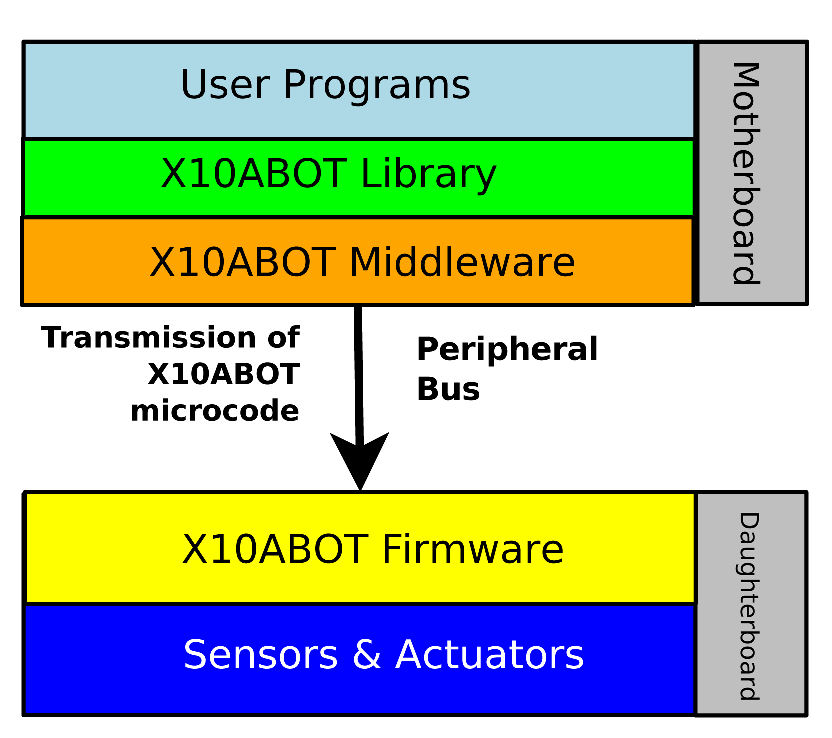
\includegraphics[width=0.7\columnwidth]{Figures/system.pdf}
	    \caption{The \xten software architecture}
	  \end{center}
	\end{figure}
	
	


	% subsubsection the_motherboard_library (end)
	\subsubsection{Application Software} % (fold)
	\label{ssub:application_software}
	Code written by users that takes advantage of the features of the \xten architecture to complete a particular task is considered to be application software. The main purpose for creating a robotics framework is to allow the end user to have a gratifying experience when developing software for their robotics project. We wanted to provide the user with the tools that will allow them to build more interesting robotics projects, without the usual limitations of scale or complexity that may follow. 
	
	We used Arduino's Processing language as our choice for the implementation of the framework. It is know to be very easy to learn and use and also has a supporting IDE that allows the user to get up and started in a short period of time. 
	Applications will be written in a C-like syntax and compiled to run on an Arduino board. This is a familiar interface for many roboticists because Arduino is a very common robotics development platform.
	% subsubsection application_software (end)
	
	\subsubsection{The Daughterboard Firmware} % (fold)
	\label{ssub:the_daughterboard_firmware}
	The daughterboard firmware allows it to provide a standard interface from all daughterboards to their motherboard. All instructions to control or access sensors and actuators are communicated to it via the peripheral bus. These instructions are written as microcode abstractions of the hardware and need to be translated to actual assertions on the devices. Each abstracted command in the motherboard's \xten Library is translated into one or more microcode hardware instructions. Microcode instructions are carried out sequentially by the daughterboards to manipulate the physical hardware components that are attached to their ports. The microcode instructions define a universal set of hardware operations. When these are logically put together, they can control virtually any typical robotics sensor or actuator.
		The microcode instructions specified for daughterboards, provide different means of interacting with each port (see Table~\ref{tab:microcode}).
	The firmware on the daughterboards will interpret these instructions and execute hardware procedures. These instructions are asserted to the standard sensor and actuator ports which are composed of pins, each with their specific purpose. Sensors and actuators are connected to their respective ports and respond to the assertions placed upon them by the daughterboard.
	
	\begin{table}[h] 
        \centering
          \scriptsize {%            
	      \begin{tabular}{|l|l|l|}
            \toprule
	        \multicolumn{3}{c}{\textbf{Microcode Instructions}} \\\hline
            \textbf{Category} & \textbf{Input/Output} & \textbf{Data}\\\hline
            Digital I/O  & Read/Write & HIGH/LOW \\\hline
            Analogue & Read & n/a \\\hline
            PWM & Write & Frequency and Duty Cycle \\\hline
            \multicolumn{3}{c}{Unimplemented Features.} \\\hline
            I$^{2}$C & Read/Write & Serial Data \\\hline 
            RS-232 & Read/Write & Serial Data \\\hline 
            Watch & Rising/Falling Edge & Threshold Value\\\hline 
            Watch & Threshold & Greater/Less than\\\hline 
            \end{tabular} 
            }
	  \caption{The complete set of hardware operations supported by the
	    microcode interface to the daughterboards as well as a few planned features.}
	  \label{tab:microcode}
	\end{table}
	\normalsize
	
 The microcode instructions are a universal set of hardware operations restricted to the types of sensors and actuators that are in common use (e.g. analogue, digital, serial, PWM). If a future sensor or actuator should use an incompatible operation, then a firmware upgrade which would include the new microcode instructions would have to be developed in order to interface with it (assuming that it could be made to be hardware compatible with the port). The microcode instructions are made to be very generic, ensuring compatibility with as many sensors and actuators as we could find at the time of design.

	
	The motherboard implements a number of functions that allow the libraries to utilise microcode instruction in the development of device libraries. These instructions are passed to the daughterboard were they are interpreted and executed. Listing ~\ref{code:micro} shows a few of the microcode instructions used in the \xten library and their related parameters.
	
	\begin{listing}
		\footnotesize
		\begin{minted}[bgcolor=bg,baselinestretch=1,frame=lines,framesep=2mm,label={Microcode Functions }]{c}
	

/**
 * @param  byte  state  The state of the digital pin, HIGH(2), LOW(1), INPUT(0)
 * @param  byte  db_address The daughterboard address , 0 for motherboard 
 * @param  byte  port_number The daughter board's port number
 * @param  byte  pin_select The I/O pin selection on the port, A(0) or B(1)
 * @param  byte  pwm_select The PWM pin selection on the port  A(0) or B(1)
 * @param  byte  duty_cycle Specify the duty cycle between 0 and 255
*/
void digitalOut(byte state, byte db_address, byte port_number, byte pin_select);
byte digitalIn(byte db_address, byte port_number, byte operation);
void pwm(byte pwm_select, byte db_address, byte port_number, byte duty_cycle);
int analog(byte db_address, byte port_number);

		\end{minted}
		\caption{Example of the \xten microcode instructions used in the Library.} \label{code:micro}
	\end{listing}

	For every event on the daughterboard that is to be triggered, a microcode instruction is sent from the motherboard. The format of the instructions are as follows: The first four bits of the first byte define the instructions to be executed and the next four bits define the specific operation for that instruction. The third byte specifies the daughterboard address and the fourth byte has seven bits for the port number and one bit for the pin selection. Each transmitted instruction has a a sequence number that that is assigned to each microcode instruction in the sequence that it is executed. Some instructions require additional data to complete its operations. The microcode format provides a sequence of data bytes that can be of arbitrary size, it is used in operations where a lot of data may be transmitted e.g RS-232. Table~\ref{tab:mc-structure} shows the structure of a typical microcode instruction.
	\begin{table}[h] \scriptsize {%
	    \newcommand{\mc}[3]{\multicolumn{#1}{#2}{#3}} 
	    \begin{center}
	      \begin{tabular}{|lll|}\hline %\mc{3}{|c|}{\textbf{}} \\\hline
	        \mc{1}{|l|}{Byte 1:} & \mc{1}{l|}{1111XXXX} & \mc{1}{l|}{FUNCTION BYTE}
	        \\\hline \mc{1}{|l|}{Byte 1:} & \mc{1}{l|}{XXXX1111} & OPERAND BYTE
	        \\\hline \mc{1}{|l|}{Byte 2:} & \mc{1}{l|}{11111111} & D.B. SELECTION
            \\\hline \mc{1}{|l|}{Byte 3:} & \mc{1}{l|}{1XXXXXXX} & PORT TYPE
	        \\\hline \mc{1}{|l|}{Byte 3:} & \mc{1}{l|}{X111111X} & PORT SELECTION
			 \\\hline \mc{1}{|l|}{Byte 3:} & \mc{1}{l|}{XXXXXXX1} & PIN SELECTION
			 \\\hline \mc{1}{|l|}{Byte 4:} & \mc{1}{l|}{XXXXXXX1} & FUNCTION SEQUENCE NUMBER
	        \\\hline \mc{1}{|l|}{Byte(s) 4+n} & \mc{1}{l|}{11111111 } & DATA
	        BYTES; n\texttt{>} 0
	        \\\hline \end{tabular}
	    \end{center} }
	  \caption{Byte layout for transmitted microcode} \label{tab:mc-structure}
	  
	\end{table}
	\normalsize
	
	Code example~\ref{code:instr} shows how microcode instructions are used to compose a particular robotics instruction in the \xten architecture. Here the method named \textbf{``on''} is defined for the Actuator class. The \textbf{power} parameter is passed as an argument to the function. For negative and positive values of \textbf{power}, separate actions are taken. the same microcode operations are executed but with different parameters.
	\begin{listing}
		\footnotesize
		\begin{minted}[bgcolor=bg,baselinestretch=1,frame=lines,framesep=2mm,label={Robot Instructions}]{c}
void Actuator::on(byte power){
  if (power>0)
  {
    actuator.pwm(A, _db, _port, 255*power/100);
    actuator.digitalOut(HI,_db,_port,A);
    actuator.digitalOut(LO,_db,_port,B);
  }
  else{
    actuator.pwm(A, _db, _port, 255*abs(power)/100);
    actuator.digitalOut(LO,_db,_port,A);
    actuator.digitalOut(HI,_db,_port,B);
  }
}
		\end{minted}
		\caption{Example of the a robotic instruction which is comprised of microcode operations.}\label{code:instr}
	\end{listing}
	
	
	The purpose of the daughterboard is to interpret these high-level instructions from the motherboard and execute them on the respective sensor or actuator irrespective of the hardware specifics of the daughterboard. This ensures that high level language instructions sent from the motherboard remains platform independent.
	
	
	% subsubsection the_daughterboard_firmware (end)
	
	\subsubsection{Middleware} % (fold)
	\label{ssub:middleware}
	Bakken et al.~\parencite{bakken2001middleware} defined middleware as follows: ``a class of software technologies designed to help manage the complexity and heterogeneity inherent in distributed systems. It is defined as a layer of software above the operating system but below the application program that provides a common programming abstraction across a distributed system.'' The portion of the \xten software architecture that performs the role of middleware does so by providing the motherboard with a level of abstraction and seamless communication with the daughterboards. The middleware handles communication between devices without exposing the details of the protocol or its requirements and the details of the systems hardware on either end. In fact the middleware is used to determine what type of communication medium and protocol is appropriate and creates a standard platform independent interface for interaction. In other words, The middleware just simply presents a standard interface that communicates data and instructions between both the motherboard and daughterboard.
	In a review of popular robotics middleware, Kramer~\parencite{kramer} cites some major advantages which are applicable to the \xten architecture. He states that it aids in software modularity, which is an intentional design objective. The middleware allows for pluggable libraries at the motherboard level which are ignorant of the actual hardware implementations. This accomplishes the platform independence, and portability that Kramer found to be a common attribute of most robotics middleware.
	
	The aspect of the \xten architecture that transports the microcode from the libraries of the motherboard to the interpreter of the daughterboard is considered to be our middleware. Each microcode instruction formats the byte string as described in Table ~\ref{tab:mc-structure}. The microcode then performs one or more of a series of dispatch and request events between the motherboard and the daughterboard. The daughterboard also initiates data transfers as well for certain special cases. All these operations are managed by the middleware. 
\begin{listing}
\footnotesize
{\fontsize{8}{6}\selectfont
\begin{minted}[bgcolor=bg,baselinestretch=1,frame=lines,framesep=2mm,label={Robot Instructions}]{c}

void X10ABOT_MB::digitalOut(byte state, byte db_address, byte port_number, byte pin_select){
  byte microcode[] = {FN_IO+state,db_address,((port_number-1)<<1)+pin_select,incr_instr_seq()};
  dispatch(microcode, sizeof(microcode));

}

byte X10ABOT_MB::digitalIn(byte db_address, byte port_number, byte pin_select){
  byte seq_num = incr_instr_seq();
  byte microcode[] = {FN_IO+IN,db_address,((port_number-1)<<1)+pin_select,seq_num};
  dispatch(microcode, sizeof(microcode));
  delay(50);
  return requestHandler(microcode, 2,seq_num);
}

void X10ABOT_MB::pwm(byte pwm_select, byte db_address, byte port_number, byte duty_cycle){
  byte microcode[] = {FN_PWM,db_address,((port_number-1)<<1)+pwm_select,incr_instr_seq(),duty_cycle};
  dispatch(microcode, sizeof(microcode));
}

\end{minted}
}
\caption{Example of the a robotic instruction which is comprised of micro-code operations.} 
\end{listing}	

The dispatch and request events are used to pass data across the peripheral bus.
	% subsubsection middleware (end)
	
	\subsubsection{Extending the Library} % (fold)
	\label{ssub:extending_the_library}
	
	To allow for easy extensibility and to support new hardware, the X10ABOT software architecture was designed to allow user extensible libraries. A library defines a set of microcode instructions used to control a hardware device.
	
	New types of sensors and actuators can be supported by adding them as a device library on the the \xten motherboard. Creating a new device specification can be done without the need to understand any low level device specific coding, since all the configurations are abstracted for easier programming. Extensibility is therefore achieved through high-level abstraction of low level hardware components.
	The \textbf{X10} in \xten which stands for extensibility, is one of the key design goals for the architecture. Extensibility defines the ability of the platform to support a vast variety of sensors and actuators with the inherent ability to support new or previously unsupported peripherals. This ability is a significant part of the core framework design. Both the hardware and software allow for inclusion for new and cutting edge technologies by utilising the simple idea of composition of low level microcode instructions. Many seemingly complex protocols or devices operate using only a few simple fundamental electronic operations defined by our microcode instructions. By creating a set of instructions that utilise these fundamental operations, any composite methods can be formed to complete most electronic tasks. For example: to operate an h-bridge, to control a DC motor, this requires a particular set of configurations of the digital I/O pins in their HI or LOW state, the configurations determine the operating mode: forward, reverse or stop. It may also require a pulse width modulation input to determine the motor's speed. These could be composed as a single library for the device. The \xten system architecture was designed to facilitate device libraries which operate in a similar sense as hardware drivers for computer peripherals. A driver typically communicates with the device through a communication subsystem to which the hardware connects.	
	% subsubsection extending_the_library (end)
	
	\subsubsection{Multitasking} % (fold)
	\label{ssub:multitasking}
	
	Another major aspect of the software system is its ability to execute simultaneous tasks. This was provided by the LEGO\textregistered Mindstorms\textregistered NXT platform and implemented in the X10ABOT robotics platform using the FreeRTOS real time scheduler. FreeRTOS is a tried and tested open source system which offers a very fast and efficient means of handling multiple tasks and timing operations.
	% subsubsection multitasking (end)
	
	\subsubsection{The X10ABOT LEGO VM} % (fold)
	\label{ssub:the_x10abot_lego_vm}
	There has been significant work toward the creation of a LEGO\textregistered Mindstorms\textregistered NXT virtual machine which will operate on top on the X10ABOT Library. User program code in the form of bytecode will be interpreted and executed with equivalent library commands. Many of the limitations in the hardware of the NXT are not enforced in its bytecode, therefore it may have the ability to utilise the extra sensors and actuator ports provided by the X10ABOT Library.
	% subsubsection the_x10abot_lego_vm (end)
	
% subsection the_software_architecture (end)

% section the_architecture (end)

\section{The Arduino Implementation} % (fold)
\label{sec:the_arduino_implementation}
\xten is a robotics architecture that is indifferent to any particular hardware system. We endeavoured to create an architecture that had very few hardware specific restrictions that would force the developer to chose one hardware platform over another. We also tried to create an architecture that was capable of running on systems as simple as 8-bit micro-controllers. What we found was that the majority of hobbyist robotics and robots used in school competitions tended to use 8-bit microcontrollers. However, many of the major notable robotics architectures were built on top of a full featured 32 or 64-bit processing systems~\parencite{Elkady2012}. The architecture should however be able to scale up to a full scale 32 or 64-bit computer. This will allow for more complex programs to be written with more processor and hardware intensive operations. The most basic requirements for any implementation of the \xten architecture is a microprocessor which has the ability to perform digital and analogue input and output. In this case, one controller will operate as both motherboard and daughterboard. In order to support external daughterboards, each microcontroller must have support for the \iic protocol in addition to the minimum requirements listed above.

The Arduino embedded system framework is a very active project, and it is notable for keeping at the cutting edge of embedded development. The framework is platform independent and currently deployed on a variety of processors including Atmel's AVR 8-bit and 32-bit ARM processors. There are even a few other companies including Microchip who have adopted the Arduino framework for their 32-bit processors as well. 
The \xten software was written with the Processing language supported by Arduino which is a derivative of C++. This allowed us to take advantage of many of C++'s high level language features including class hierarchy which is the basis of how development for the motherboard libraries are done. Arduino also comes with a cross platform IDE that allows development on all the major operating systems.

The Arduino platform provides very inexpensive hardware that can be used for both motherboard and daughterboard. They were designed for physical add-ons called shields which are convenient connection boards that can host auxiliary circuitry like port headers, external power and H-bridges.

% section the_arduino_implementation (end)

